
\chapter{Anforderungserhebung}\label{sec:chapter5}
In diesem Kapitel werden die Anforderungen an den in Kapitel 5 folgenden Vergleich der imperativen und deklarativen Modellierung für SE-Prozessmodelle erhoben. Hierfür werden zunächst in Kapitel 4.1 die Vergleichskriterien vorgestellt und erläutert. 

\section{Vergleichskriterien}\label{sec:chapter5:Vergleichskriterien}

Bisher gibt es nur wenige Arbeiten, welche sich mit deklarativen Prozessmodellierungssprachen und insbesondere mit dem Vergleich von imperativen und deklarativen Prozessmodellierungssprachen beschäftigen. Aus diesem Grund soll in der vorliegenden Arbeit ein Vergleich der Anwendbarkeit zwischen deklarativen und imperativen Prozessmodellierungssprachen im Kontext von Softwareentwicklungsprozessen durchgeführt werden. Hierbei soll die Eignung der beiden Prozessmodellierungssprachen für die Modellierung beurteilt werden. Weiterhin sollen die Stärken und Grenzen der beiden Modellierungssprachen aufgezeigt werden und es soll dadurch herausgefunden werden, ob eine der beiden Modellierungssprachen über eine bessere Anwendbarkeit bei der Modellierung verfügt als die andere \cite{list2006evaluation}.\newline
Hierfür sollen die imperativen und deklarativen Prozessmodelle, welche für die drei Softwareentwicklungsprozesse Scrum, Open UP und V-Modell-XT erstellt werden im Hinblick auf verschiedene Vergleichskriterien untersucht werden. Da es sich bei Scrum um ein leichtgewichtiges Softwareentwicklungsprozessmodell, beim V-Modell XT um ein schwergewichtiges Softwareentwicklungsprozessmodell und bei Open UP um ein Softwareentwicklungsprozessmodell handelt, welches sich in der Mitte zwischen leichtgewichtig und schwergewichtig befindet, eignen sich diese drei besonders gut, zum Vergleichen der imperativen und deklarativen Modellierung für unterschiedlich große Matamodelle. Außerdem liegen den in imperativer und deklarativer Modellierungssprache zu erstellenden Prozessmodellen so jeweils die gleichen Metamodelle zugrunde, was eine objektive Bewertung für den Vergleich gewährleistet \cite{list2006evaluation}. \newline

Es sollen die imperativen und deklarativen Modellierungssprachen im Hinblick auf deren Erfüllung der in Kapitel 3.1.1 vorgestellten \textit{Grundsätze ordnungsgemäßer Modellierung} untersucht werden, da durch deren Einhaltung die Qualität, Klarheit und Konsistenz der Prozessmodelle gesichert wird \cite{freund2007}. Somit lässt sich hierdurch die Eignung der beiden Prozessmodellierungssprachen sehr gut überprüfen. Denn falls eine von beiden Prozessmodellierungssprachen die Modellierungsgrundsätze wesentlich schlechter einhalten kann, als die andere, so ist sie zum Modellieren deutlich weniger geeignet, da die hierdurch entstandenen Prozessmodelle geringere Qualität, Klarheit und Konsistenz aufweisen. Hierfür werden nachfolgend die erstellten Prozessmodelle im Hinblick auf \textit{Richtigkeit}, \textit{systematischen Aufbau}, \textit{Relevanz}, \textit{Klarheit}, \textit{Wirtschaftlichkeit} und \textit{Vergleichbarkeit} verglichen. Hierfür werden nachfolgend für jeden Modellierungsgrundsatz verschiedene Kriterien festgelegt, mit deren Hilfe die Einhaltung der Modellierungsgrundsätze für die jeweilige Modellierungssprache überprüft wird. \newline

\subsection{Richtigkeit}
Die Richtigkeit der Prozessmodelle soll verglichen werden. Hierbei soll die syntaktische und semantische Richtigkeit der Prozessmodelle untersucht werden. \newline


\subsubsection{A 1.1}

Die sysntaktische Korrektheit wird dahingegend untersucht, ob sich die jeweiligen Modelle unter Einhaltung der Modellierungsregeln der jeweiligen Prozessmodellierungssprache erstellen lassen. Dies wird mit Hilfe der Modellierungstools Signavio und Declare durchgeführt. Beide Programme verfügen über eine automatische Überprüfung der syntaktischen Korrektheit der dort erstellten Modelle. \newline

\subsubsection{A 1.2}

Bei der semantischen Korrektheit der Prozessmodelle wird verglichen in wie weit die mit deklarativer bzw. imperativer Prozessmodellierungssprache erstellten Prozessmodelle dem zugrunde liegenden Metamodell gegenüber vollständig und konsistent sind. Denn falls wesentliche Aspekte des Metamodells nicht darstellbar sind, leidet der Nutzen des Prozessmodells erheblich. Es wird somit überprüft, ob eine der beiden Prozessmodellierungssprachen die Struktur des Metamodells und das dort beschriebe Verhalten besser abbildet als die andere. Insbesondere wird hier untersucht, ob es Grenzen in der Darstellbarkeit der abzubildenden Aspekte des Metamodells gibt \cite{journals95, becker2012prozessmanagement}. \newline


\subsection{Systematischer Aufbau}

 Da nicht alle Informationen, wie z.B. Daten und Funktionen in einem Prozessmodell abgebildet werden können, ist die Integration anderer Sichten in das Prozessmodell sehr wichtig, um wirklich alle Informationen aus dem Metamodell abbilden zu können. Hier können Rückschlüße auf die Eignung zur Modellierung gezogen werden und eventuelle Grenzen der Prozessmodellierungssprache aufgezeigt werden \cite{journals95, freund2007, becker2012prozessmanagement,koch2011}.


\subsubsection{A 2.1}
Um den systematischen Aufbau der imperativen und deklarativen Prozessmodelle zu vergleichen, werden die Prozessmodelle dahingehend untersucht, in wie weit sie die Integration anderer Sichten in das Prozessmodell unterstützen und sie Verweise auf bestehende Datenmodelle zulassen. 

\subsection{Relevanz}

Beim Vergleich der Relevanz der Prozessmodelle werden die mit BPMN bzw. ConDec modellierten Prozessmodelle dahingehend verglichen in wie weit es möglich ist die Prozessmodelle mit den minimal relevanten Informationen zu erstellen. Hier kann wiederum die Eignung der beiden Prozessmodellierungssprachen sehr gut verglichen werden, da falls mit einer Prozessmodellierungssprache nicht alle minimal relevanten Informationen des Metamodells abgebildet werden können, ist diese nicht zum Modellieren geeignet \cite{journals95, freund2007,reinshagen2009}. 

\subsubsection{A 3.1}

Hier soll somit ein direkter Vergleich zwischen den imperativen und deklarativen Prozessmodellen durchgeführt werden. Anhand von diesem soll festgestellt werden, ob in einer von beiden Prozessmodellierungssprachen mehr Informationen zum Metamodell abgebildet werden können, als in der anderen.\newline

\subsection{Klarheit}


Die Prozessmodelle, welche jeweils in imperativer und deklarativer Prozessmodellierungssprache erstellt werden, sollen im Hinblick auf ihre Klarheit untersucht werden. Hierbei soll festgestellt werden, ob es wesentliche Unterschiede bei der Verständlichkeit der Prozessmodelle gibt, wenn diese in imperativer, bzw. deklarativer Prozessmodellierungssprache erstellt wurden. Denn fehlende Verständlichkeit eines Prozessmodells führt dazu, dass das Prozessmodell wenig Nutzen bringt. 


\subsubsection{A 4.1}
Es soll die Anzahl an Gateways in BPMN und Constraints in ConDec betrachtet werden. Da alle Gateways in BPMN und alle Constraints in ConDec eine unterschiedliche Sematik haben und diese jeweils verstanden werden muss, kann sich eine hohe Anzahl an Gateways, bzw. Constraints negtiv auf die Verständlichkeit auswirken \cite{gruhn2006adopting, thesis_maja}. \newline
In der Studie \cite{gruhn2006adopting} wurden Metriken über den geistigen Aufwand entwickelt, welcher für das Verständnis von BPMN-Notationselementen notwendig ist. Den einzelnen Notationselementen werden dort verschiedene geistige Gewichtungen zugewiesen. Ein Sequenzfluss hat auf Grund des geringen geistigen Aufwandes beim Verstehen eine geistige Gewichtung von 1. Das Exklusive Gateway hat eine geistige Gewichtung von 2, falls es nur zwei ausgehende Kanten hat. Bei drei oder mehr ausgehenden Kanten hat es eine geistige Gewichtung von 3. Das Parallele Gateway hat eine geistige Gewichtung von 4. Einem Inklusiven Gateway wird sogar eine geistige Gewichtung von 7 zugeschrieben \cite{gruhn2006adopting}.\newline
Leider existieren derzeit noch keine Metriken über den geistigen Aufwand beim Verstehen der einzelnen Constraints bei ConDec. Jedoch gibt es bereits Studien (\cite{thesis_maja,haisjackl2014understanding}), welche sich anderweitig mit dem Verstehen von deklarativen Prozessmodellen auseinandergesetzt haben. Da die Existenz-Constraints relativ einfach zu verstehen sind, werden sie beim Vergleich in Kapitel 5 mit den Sequenzflusselemeneten gleichgesetzt und haben somit auch in etwa eine geistige Gewichtung von 1. \newline
Da die Constraints in ConDec genau wie die Gateways in BPMN Patterns darstellen, müssten sie ebenfalls alle Werte für die geistige Gewichtung zwischen 2 und 7 annehmen. Da die Constraints jedoch nicht direkt den Gateways in BPMN zugeordnet werden können und sich somit die geistigen Gewichtungen der Gateways nicht auf die Constraints übertragen lassen wird im Vergleich in Kapitel 5 nur die jeweilige Anzahl an Gateways in BPMN mit der Anzahl an Constraints im ConDec-Modell verglichen. \newline
Zudem wird auch die Anzahl an unterschiedlichen Gateways/Constraints betrachtet. Denn sowohl bei BPMN, als auch bei ConDec wurde in Studien herausgefunden, dass gerade die Kombination von vielen verschiedenen Gateways/Constraints einen sehr großen negativen Einfluß auf das Verstehen hat \cite{gruhn2006adopting, thesis_maja,haisjackl2014understanding}. \newline

\subsubsection{A 4.2}

Weiterhin soll auch die Anzahl der Elemente insgesamt, welche zur Erstellung der Modelle notwendig sind verglichen werden, denn Prozessmodelle werden mit steigender Anzahl an Elementen unverständlicher \cite{leimeister2012, journals95, freund2007,reinshagen2009}. 


\subsubsection{A 4.3}
Zudem soll untersucht werden, ob bei dem mit ConDec erstellten Modell ein klarer Einstiegspunkt mit Hilfe des Init-Constraints dargestellt werden kann. Das Init-Constraint kann bei ConDec nur einer einzigen Aktivität im Modell zugewiesen werden. Kommen mehrere Aktivitäten als Einstiegspunkt im Modell in Frage, so lassen sich diese in ConDec nicht klar kennzeichnen. Es existieren Studien darüber, dass sich dies negativ auf das Verständnis von ConDec Modellen auswirkt \cite{haisjackl2014understanding}. \newline

\subsubsection{A 4.4}
Weiterhin soll hier untersucht werden, ob es wesentliche Unterschiede in der Verständlichkeit der imperativen und deklarativen Prozessmodellen gibt, in Abhängigkeit der Größe des Prozessmodells. Hierbei kann die Eignung der jeweiligen Modellierungssprache sehr gut festgestellt werden, da sie im Falle von schwerer/fehlender Verständlichkeit nicht zum Modellieren geeignet ist. Falls es Unterschiede in der Verständlichkeit der Prozessmodelle in Abhängigkeit der Größe des zugrunde liegenden Metamodells gibt, lassen sich hierbei Rückschlüsse auf die Eignung der Prozessmodellierungssprache in Bezug auf große/kleine Modelle ziehen \cite{leimeister2012,journals95, freund2007,reinshagen2009, becker2012prozessmanagement,koch2011,bpm07,thesis_maja}.


\subsection{Wirtschaftlichkeit der Prozessmodelle}

Hier soll untersucht werden, ob sich der Aufwand für die Modellierung bei den beiden Modellierungssprachen erheblich voneinander unterscheidet, da wenn die Erstellung eines Prozessmodells mit einem zu hohen Aufwand verbunden ist, obwohl der spätere Nutzen des Prozessmodells erheblich geringer ist, ist die Modellierung nicht sinnvoll. Hier kann die Eignung zur Modellierung der Prozessmodellierungssprachen sehr gut verglichen werden, denn falls der Aufwand für die Modellierung für eine der beiden Prozessmodellierungssprachen weitaus höher ist, eignet sich die Prozessmodellierungssprache mit dem sehr viel höherem Aufwand nicht für die Modellierung.\newline

\subsubsection{A 5.1}
Hier wird einerseits die Anzahl der Elemente insgesamt, welche zur Modellierung der Prozesse notwendig sind miteinander verglichen.

\subsubsection{A 5.2}
 Weiterhin wird die Anzahl von Gateways in BPMN mit der Anzahl von Constraints in ConDec miteinander verglichen und auch die Anzahl unterschiedlicher Gateways/Constraints. Da bei der Verwendung von Gateways/Constraints für den Modellierer ein höherer geistiger Aufwand notwendig ist und somit auch ein größerer Aufwand für das Modellieren, kann sich dies negativ auf die \textit{Wirtschaftlichkeit} auswirken. Weiterhin sind komplexere Modelle auch fehleranfälliger, d.h. wenn der Modellierer einen höheren geistigen Aufwand beim Modellieren leisten muss, ist es auch wahrscheinlicher, dass ihm Fehler beim Modellieren passieren \cite{freund2007, journals95, leimeister2012,mendling2010seven}.


\subsection{Vergleichbarkeit}
Bei der Vergleichbarkeit der Prozessmodelle wird untersucht, ob die in imperativer, bzw. deklarativer Prozessmodellierungssprache erstellten Prozessmodelle, welchen die gleichen Metamodelle zugrunde liegen, trotzdem vergleichbare Prozessmodelle darstellen.

\subsubsection{A 6.1}
Weiterhin wird die Vergleichbarkeit in Bezug auf das Ausführungsverhalten der imperativen und deklarativen Prozessmodelle durch Ausführung der Modelle in den Modellierungstools Siganvio und Declare nach der Modellierung überprüft. Hier werden die Pfade, welche im jeweiligen Modell durchlaufen werden können miteinenader verglichen und somit wird sichergestellt, dass das Verhalten der Modelle gleich ist, wenn bei beiden Modellen die gleichen Pfade möglich sind.

\subsubsection{A 6.2}
Außerdem wird hier die Größe der jeweiligen Prozessmodelle als Vergleichskriterium herangezogen. Hier wird die Gesamtanzahl der notwendigen Elemente zur Darstellung des Prozessmodells verglichen. Es soll festgestellt werden, ob bei Verwendung einer imperativen oder deklarativen Prozessmodellierungssprache wesentlich mehr Elemente zur Darstellung des gleichen Prozesses notwendig sind indem die Anzahl der verwendeten Aktivitäten und Patterns verglichen wird \cite{leimeister2012, journals95, freund2007,reinshagen2009}.

 \subsubsection{A 6.3}
Es wird hier somit insbesondere untersucht, ob die Abstraktionsgrade der Prozessmodelle sich wesentlich voneinander unterscheiden. 


Eine Übersicht über die Modellierungsgrundsätze und die jeweiligen Vergleichskriterien bietet Abbildung \ref{fig:TabelleKriterien}.

\begin{figure}[!htbp]
\begin{center}
  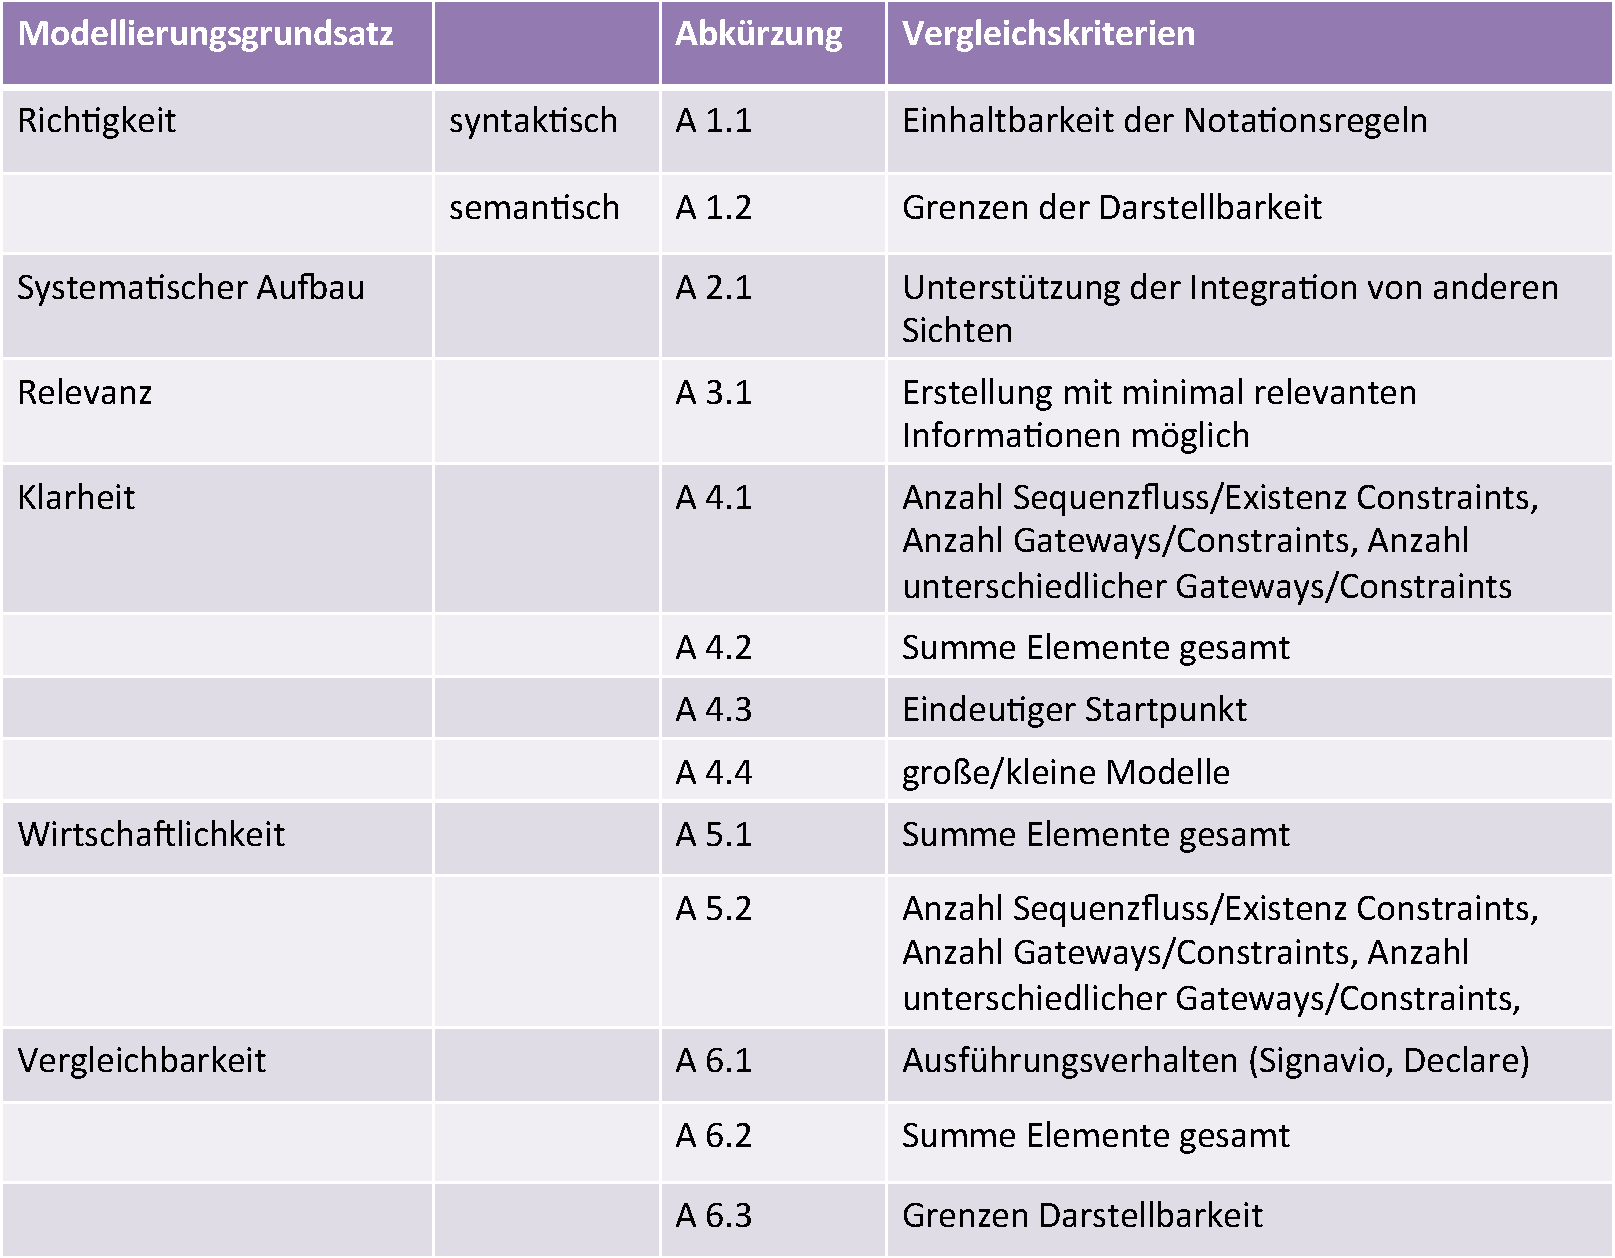
\includegraphics[width=\textwidth]{TabelleKriterien} %pdf, jpg, png...
  \caption{Übersicht Vergleichskriterien}
  \label{fig:TabelleKriterien}
\end{center}
\end{figure}








